\documentclass{article}

% Language setting
% Replace `english' with e.g. `spanish' to change the document language
\usepackage[greek,english]{babel}
\newcommand{\en}{\selectlanguage{english}}
\newcommand{\gr}{\selectlanguage{greek}}
% other packages
\usepackage{graphicx}
\usepackage[colorlinks=true, allcolors=blue]{hyperref}
\usepackage[T1]{fontenc}
\usepackage[utf8]{inputenc}
\usepackage{tabularx,ragged2e,booktabs,caption}
\newcolumntype{C}[1]{>{\Centering}m{#1}}
\renewcommand\tabularxcolumn[1]{C{#1}}
\usepackage[letterpaper,top=2cm,bottom=2cm,left=3cm,right=3cm,marginparwidth=1.75cm]{geometry}
\usepackage{infwarerr}


\title{\textbf{FIRST ASSIGNMENT IN MICROECONOMETRICS}}

\author{onoma , A.M.: \\
	onoma, A.M.: \\
	onoma, A.M.: \\
	onoma, A.M.: }

\date{November, 2022\\
	University of Patras\\
	Department of Economics\\
	MSc Applied Economics and Data Analysis}

\begin{document}
	
	\centering
	%pinakas gia to thema 1
	\large{\textbf{THEMA 1}}
	
	\vspace {0.5\baselineskip}
	
	grapse kati
	
	
	
	\captionof{table}{Titlos} \label{tab:title} 
	
	\begin{tabular}{|c |c |c |c |c |}
		\toprule
		Variable & Mean & Std.dev. & Min & Max \\ 
		\midrule
		inlf & 0.5683931 & 0.4956295 & 0 & 1\\
		hours & 740.5764 & 871.3142 & 0 & 4950 \\
		kidslt6 & 0.2377158 & 0.523959 & 0 & 3\\
		kidsge6 & 1.353254 & 1.319874 & 0 & 8\\\
		age & 42.53785 & 8.072574 & 30 & 60\\\
		educ & 12.28685 & 2.280246 & 5 & 17\\\
		wage & 4.177682 & 3.310282  & 0.1282 & 25\\\
		repwage & 1.849734 & 2.419887 & 0 & 9.98\\\
		hushrs & 2267.271 & 595.5666 & 175 & 5010\\\
		husage & 45.12085 & 8.058793 & 30 & 60\\\
		huseduc & 12.49137 & 3.020804 & 3 & 17\\\
		huswage & 7.482179 & 4.230559 & 0.4121 & 40.509\\\
		faminc & 23080.59 & 12190.2 & 1500 & 96000\\\
		mtr & 0.6788632 & 0.0834955 & 0.4415 & 0.9415\\
		motheduc & 9.250996 & 3.367468 & 0 & 17\\\
		fatheduc & 8.808765 & 3.57229 & 0 & 17\\\
		unem & 8.623506 & 3.114934 & 3 & 14\\\
		city & 0.6427623 & 0.4795042 & 0 & 1\\\
		exper & 10.63081 & 8.06913 & 0 & 45\\\
		nwifeinc & 20.12896 & 11.6348 & -0.0290575 & 96\\
		expersq & 178.0385 & 249.6308 & 0 & 2025\\
		\bottomrule
		
	\end{tabular} \par
	Provided by microdataset1 from Stata
	
	\vspace {0.5\baselineskip}
	
	sxolia--------------------------
	
	\vspace {0.5\baselineskip}
	
	\large{\textbf{THEMA 2}}
	
	\vspace {0.5\baselineskip}
	
	grapse kati------------------
	
	\vspace {0.5\baselineskip}
	
	\large{\textbf{THEMA 3}}
	
	\vspace {0.5\baselineskip}
	
	grapse kati-------------------
	
	\vspace {0.5\baselineskip}
	
	%istogramata
	\begin{figure}
		\centering
		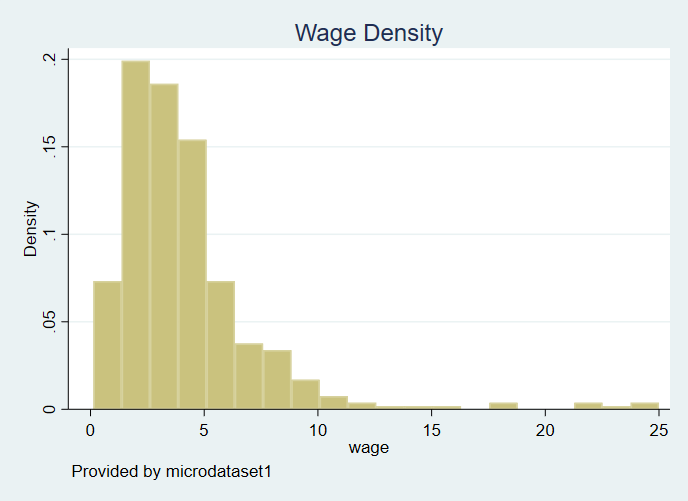
\includegraphics[width=0.5\textwidth]{Wage density.png}
		\caption{\label{fig:plot} }
	\end{figure}
	
	\vspace {0.5\baselineskip}
	
	sxolia------------------------
	
	\vspace {0.5\baselineskip}
	
	\begin{figure}
		\centering
		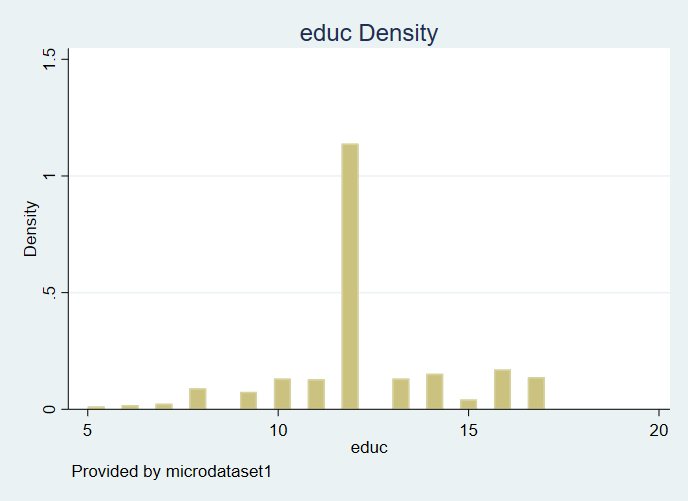
\includegraphics[width=0.5\textwidth]{educ density.png}
		\caption{\label{fig:plot} }
	\end{figure}
	
	\vspace {0.5\baselineskip}
	
	sxolia-----------------------
	
	\vspace {0.5\baselineskip}
	
	\begin{figure}
		\centering
		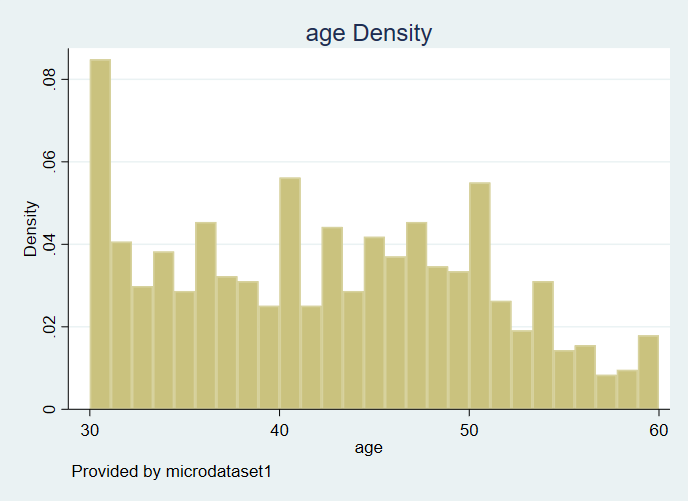
\includegraphics[width=0.5\textwidth]{age density.png}
		\caption{\label{fig:plot} }
	\end{figure}
	
	\vspace {0.5\baselineskip}
	
	sxolia----------------------
	
	\vspace {0.5\baselineskip}
	
	\begin{figure}
		\centering
		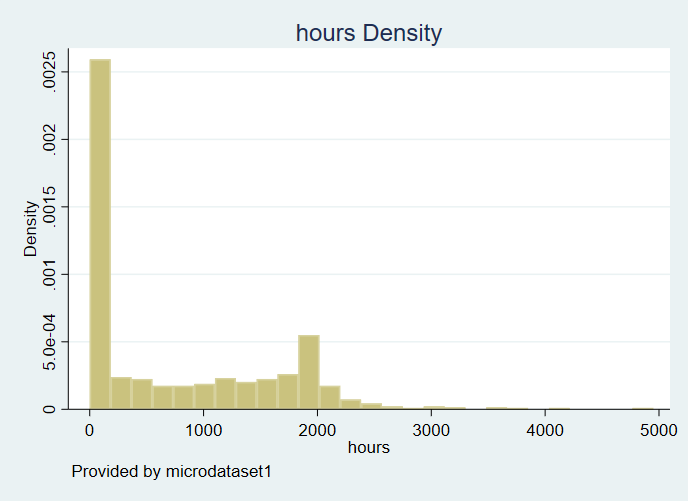
\includegraphics[width=0.5\textwidth]{hours density.png}
		\caption{\label{fig:plot} }
	\end{figure}
	
	\vspace {0.5\baselineskip}
	
	sxolia------------------------
	
	\vspace {0.5\baselineskip}
	
	\begin{figure}
		\centering
		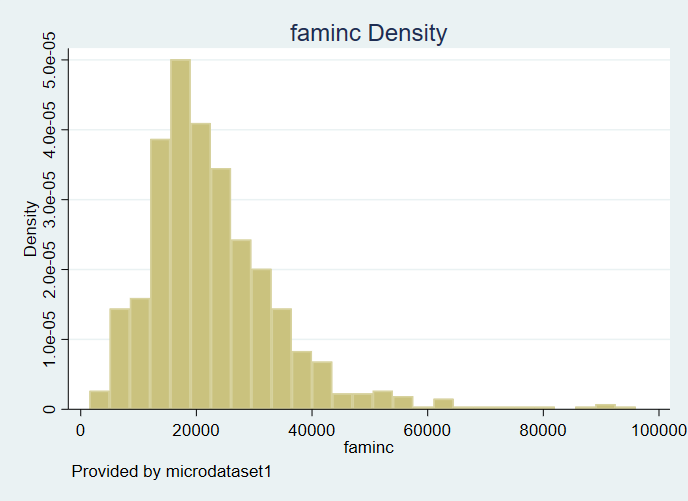
\includegraphics[width=0.5\textwidth]{faminc density.png}
		\caption{\label{fig:plot} }
	\end{figure}
	
	\vspace {0.5\baselineskip}
	
	sxolia------------------------
	
	\vspace {0.5\baselineskip}
	
	\begin{figure}
		\centering
		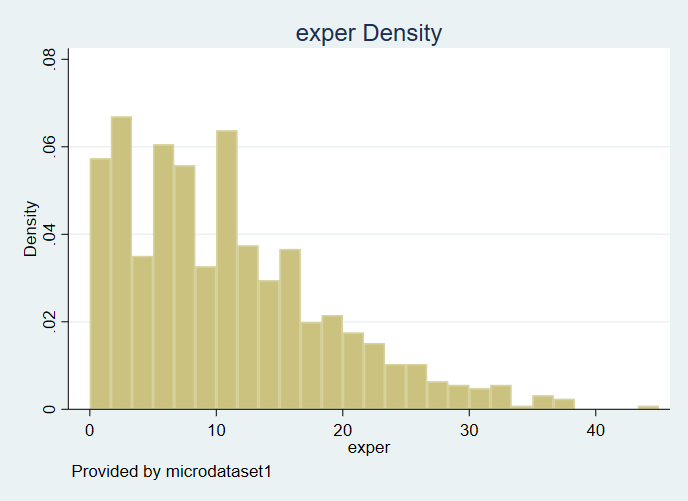
\includegraphics[width=0.5\textwidth]{exper density.png}
		\caption{\label{fig:plot} }
	\end{figure}
	
	\vspace {0.5\baselineskip}
	
	sxolia----------------------
	
	\vspace {0.5\baselineskip}
	
\end{document}